% IEEE standard conference template; to be used with:
%   spconf.sty  - LaTeX style file, and
%   IEEEbib.bst - IEEE bibliography style file.
% --------------------------------------------------------------------------
\documentclass[letterpaper]{article}
\usepackage{spconf,amsmath,amssymb,graphicx,listings,hyperref,array,float,epstopdf,tikz,subfig}
%\lstset{basicstyle=\ttfamily\footnotesize,numbers=left,stepnumber=2,frame=single,language=c,captionpos=b}
\usepackage[utf8]{inputenc} % UTF-8 was invented to be used.
\usetikzlibrary{automata,positioning}
\usetikzlibrary{shadows}


% Example definitions.
% --------------------
% nice symbols for real and complex numbers
\newcommand{\R}[0]{\mathbb{R}}
\newcommand{\C}[0]{\mathbb{C}}

% make document compile with \todo comments
\newcommand{\todo}[2][]{\textbf{TODO #2}}

% bold paragraph titles
\newcommand{\mypar}[1]{{\bf #1.}}

% Title.
% ------
\title{Parallel XML Query Processing using XML Stream Compression}
%
% Single address.
% ---------------
\name{Serge Balzan, Stefan Dietiker, Tobias Kaiser}
\address{Department of Computer Science\\ ETH Z\"urich\\Z\"urich, Switzerland}

% For example:
% ------------
%\address{School\\
%		 Department\\
%		 Address}
%
% Two addresses (uncomment and modify for two-address case).
% ----------------------------------------------------------
%\twoauthors
%  {A. Author-one, B. Author-two\sthanks{Thanks to XYZ agency for funding.}}
%		 {School A-B\\
%		 Department A-B\\
%		 Address A-B}todo
%  {C. Author-three, D. Author-four\sthanks{The fourth author performed the work
%		 while at ...}}
%		 {School C-D\\
%		 Department C-D\\
%		 Address C-D}
%

\begin{document}
%\ninept
%
\maketitle
%

\begin{abstract}
In the age of big data real time data processing becomes more and more
relevant. Many data sources, such as the Twitter Firehose, rely on context-free
languages, such as XML, to provide an interface for developers. Since such a 
data stream can reach a throughput, which is not feasible to process
on a single commercial/home computer, there exists a demand for high performance 
computating system in combination with a parallelizable approach to parse and query
the XML data in real time. 

Describe in concise words what you do, why you do it (not necessarily
in this order), and the main result.  The abstract has to be
self-contained and readable for a person in the general area. You
should write the abstract last.
\end{abstract}




\section{Introduction}\label{sec:intro}

In this report we describe the results of our project that was part of the
course ''Design of Parallel and High Performance Computing'' at ETH Z\"urich.
The goal of the project was to develop a parallel implementation of an important
algorithm or application, that scales well in a multicore environment. This
report describes an approach to process large XML files or data streams in
parallel using the XPath query language.

XML is most commonly used as an interoperable file exchange format and as such
is used in a wide variety of fields, from documents formats, such as Open
Document Format \todo{ref} and or XHTML \todo{ref} to various kinds of
configuration file formats. All of these applications have in common that XML is
primarily used as a general tool to persist and restore the dynamic state of an
application program.

Following the on-going trend towards big data, however, XML has also been used
to make large amounts of structured data available as high throughput streams.
One such example is Twitter Firehose which makes all user generated tweets
available trough a single XML-Stream\footnote{Twitter has changed the document
format from XML to JSON. We point out that the techniques presented in this
report can easily be adapted to work with almost any structured data exchange
format.}. Twitter Firehose reaches a throughput of up to 3 Gbps.

Most off-the-shelf are single-threaded and tailored towards the applications
mentioned above. Processing structured data at such a high throughput, however,
only becomes possible by leveraging the power of multi processor systems. As
parsing is an inherently sequential process, this requires the careful
orchestration of parallel processors.

Ideally, the data can be split into chunks, such that it can be processed independently.
In our approach we achieve this by using a compression that is agnostic of the
internal structure of the XML data. The XPath query matching is done using the
compressed data.

Our implementation focuses on XML query matching, using XPath. It is written in
C/C++ and our platform of choice is the Intel's Xeon Phi \cite{IntelXeon}, incorporating 61 cores
and 16 GB of memory. We found a scalable approach to process queries on large
XML files. Our implementation reaches a throughput of about 0.29 GB/s and offers
a big potential for optimization to the architecture at use. 

\mypar{Related work} Main inspiration of our work was \cite{Ogden2013}. Ogden et
al describe an approach to query XML data with the help of pushdown transducers.
Its core idea is to generate mappings of a start state and an end state. For
each chunk one mapping is being computed and then, when each core has finished
processing its part, they are merged according to the matching end and start
states of each chunk.

Optimally to process XML streams, deterministic automatons are used. The
compilation of XPath queries into automatons is discussed in \cite{Green2004}.


%\mypar{Motivation} Nowadays, in the age of the internet of things and social
%media, where a lot and continuous information is being generated and every
%single person has the opportunity to share their thoughts and insights, a huge
%content of valuable information is available. One of these examples is the
%Twitter Firehose, which generates an output of all tweet being made in real
%time. The data stream may reach an output rate of 3 Gbps and more on  its peak,
%therefore to process this data in real time requires high computational power.
%
%To achieve the necessary processing power, one can use a multicore chip, that
%provides several processing units, that work in parallel. While dealing with
%such a datastream or data file in sequential is trivial and straight-forward, an
%implementation in parallel is not as simple. The data formats used are mostly
%context-free languages, such as XML or JSON. To operate on the stream in
%parallel, it must be splitted into similar chunks and distributed to each core.
%Ideally, these chunks are well-formed and self-contained, such that no
%processing unit requires to exchange any information with other units. To
%generate well-formed chunks, parsing and preprocessing the data beforehand
%sequentially is necessary. As this might pose a bottleneck for parallel and
%high-performance query matching on XML data, in our approach we try to avoid any
%preprocessing on the raw data. Thus we had to find a way, in which each unit is
%able to operate on its chunk without any additional information from its peers.


\section{Background}\label{sec:background}
In this section, we first give the problem definition while simultaneously
introducing the (subset of the) XML Path Language–or XPath for short–
%TODO:Ref Xpath.
by giving small running examples.
We then give a general overview over three main design approaches for XPath
Query Processors and briefly discuss how our solution relates to these
approaches (TODO maybe not). Finally, we provide a formal description of the
push-down automatons that we use in our approach.

\subsection{XML Querying using XPath}

XPath models an XML document as a tree of nodes. Each node of an XML document
can be addressed by an path expressions. A path expression might \emph{match}
multiple nodes in an XML document.

For the purposes of this project we only consider a limited subset of path
expressions. However, we believe that the methods and concepts provided in this
report can be extended in a canonical way to support a more expressive path
expressions. The grammar rules for the subset we chose are as follows:

% TODO: syntax

Figure TODO shows two examples of XPath queries. The first and second both match
the same node.

/a/b/c
/a/*/c

\mypar{Problem Definition (informal).} Given an XML Document and a set of path
XPath expressions (as defined above), report all nodes that match any of the
given path expressions.

% TODO syntax description

\subsection{Parallel XPath Query Matching}

In general, three approaches for XML query processing can be distinguished:

\begin{enumerate}
\item XML parsing and querying,
\item XML-capable DBMS, and
\item XML stream processing using automatons.
\end{enumerate}

\mypar{XML parsing and querying.} First parsing the document, generating a DOM
tree, and then querying the resulting DOM tree seems like a natural choice. The
XML document can be split into chunks and which are then parsed in parallel.
However, in order for these chunks to be independent of each other, they must be
well-formed. This, in turn, requires a sequential pre-parsing step, which
eventually becomes a bottleneck.

Approaches for parallel DOM Tree parsers have been discussed in the literature.
For instance, in \todo{cite this other paper where they have created a tree
parser for open office documents}, ... However, this approach is only suitable
for comparatively small documents, according to the authors.

\mypar{XML-capable DBMS.}

Some relational DBMS-engines (MSQL, MySQL, MonetDB) have support for indexing
over XML documents. Using indices, the querying can be parallelized. However,
generating these indices takes up...

\mypar{XML processing with automatons.} The general structure of this approach
is simple. A parser (e.g. a SAX-parser) reads the XML document and triggers
parsing events that are handled by a (pushdown) automaton. The pushdown
automaton transitions into an accepting state if one the path expressions of the
input query matches.

One advantage of this approach is that both the parser and the automaton need to
maintain only comparatively little state. Indeed, the authors of \todo{citation}
which is the inspiration for this project, claim that it is the low memory
bandwidth requirements that make their approach better than the alternative
DOM-tree approach which they compare against.

\mypar{XML Parsing.} 

\subsection{XPath Query Matching}



%ive a short, self-contained summary of necessary
%ackground information. For example, assume you present an
%mplementation of sorting algorithms. You could organize into sorting
%efinition, algorithms considered, and asymptotic runtime statements. The goal of the
%ackground section is to make the paper self-contained for an audience
%s large as possible. As in every section
%ou start with a very brief overview of the section. Here it could be as follows: In this section 
%e formally define the sorting problem we consider and introduce the algorithms we use
%ncluding a cost analysis.

%mypar{Sorting}
%recisely define sorting problem you consider.

%mypar{Sorting algorithms}
%xplain the algorithm you use including their costs.

%s an aside, don't talk about "the complexity of the algorithm.'' It's incorrect,
%roblems have a complexity, not algorithms.


\section{Proposed System}\label{sec:yourmethod}

\subsection{Overview}

The method that we propose can be viewed as a batch processing system consisting
of four components (Figure \ref{fig:methodoverview}): the \emph{query
transformer}, the \emph{chunker}, the {tokenizer}, and the \emph{matcher}.
Figure \ref{fig:methodoverview} provides an overview.

\begin{figure}[tb]\centering
	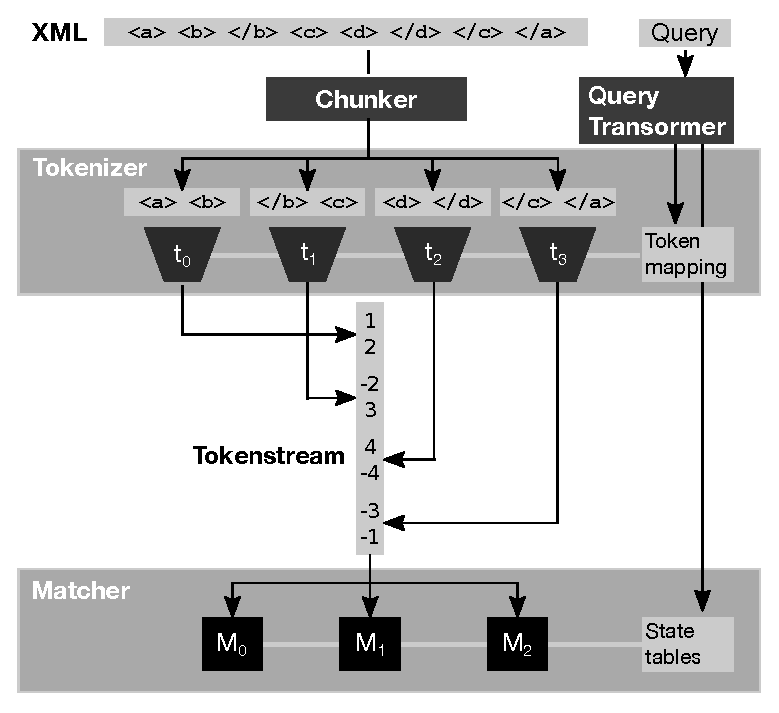
\includegraphics[width=.5\textwidth]{img/methodoverview.eps}
  \caption{Batch view of the system.}
  \label{fig:methodoverview}
\end{figure}

First, the \emph{query transformer} analyzes the query and produces a
\emph{token mapping} and set of state tables. Each state table corresponds to
one dPDA which in turn correspond to the individual path expressions.

The \emph{chunker} splits the XML streams into chunks of approximately equal
size. Individual opening or closing tag (e.g. \verb;<a>;, or \verb;</a>;) are
never split, however the structure of the XML data contained in the individual
chunks can be arbitrary.

The \emph{tokenizer} then compresses each XML chunk into a tokenstream chunk,
using the token mapping generated by the query transformer to map tag names to
token IDs. Connected together, these tokenstream chunk form the tokenstream. In
the \emph{matcher}, the push-down automatons are run in parallel over the
entire tokenstream to identify matching nodes.

The aim of our method is to reduce memory traffic in the matching phase, as the
tokenstream takes up less memory than the original XML stream. Workloads are
divided differently in the tokenizer and in the matcher. Our method is
successful if we achieve \emph{strong scaling} for the tokenizer and \emph{weak
scaling} for the matcher.

\subsection{Query Transformer}

The query transformer takes as input an XPath query which takes the form of a
text file containing one or more XPath expression. The query transformer outputs
two text files: a token mapping and a file containing the state tables of
the dPDAs, one for each path expression in the input file.

A token mapping is simply a list containing all tag names that appear in any of
the path expressions. The line number corresponds to the token ID for the tag
name on that particular line. These token numbers serve as input alphabet of
the dPDAs.

The dPDAs are generated using the methods presented in \cite{Green2004}: Each
path expression is turned into a query tree. However, as opposed to
\cite{Green2004}, we build a query tree for each individual path expression.
Based upon the query tree a non-deterministic automaton is generated which is
then transformed into a deterministic automaton using the standard power set
method described in \cite{Hopcroft2006}.

\subsection{Chunker}

The chunker splits the input XML file into chunks of approximately equal size.
The minimum size of a chunk is determined by dividing the size of the XML
document by the number of available threads in the tokenizer. The first chunk
starts the beginning of the XML stream. The start of the following chunk is
determined by adding the minimum chunk size to the current position and
searching for the next less-than-sign ('\texttt{<}')–these offsets accumulate
over all chunks, rendering the last chunk smaller than the minimum chunk size,
but we assume that the effects of this are negligible for our considerations.

\subsection{Tokenizer and Tokenstream}

The tokenizer maps tag names onto corresponding token numbers according to the
token mapping generated by the query transformer: A top-down parser parses the
XML and whenever an opening or closing tag is found, the tag name is compared
with a list of known tag names from the token mapping. For closing tags, the
token number is negated. If $n$ is the number of unique tag names contained in
the input query, all unknown opening (closing) tags, i.e. tag names that appear
in the XML stream but are not contained in the query, are mapped onto the token
number $n+1$ (or $-(n+1)$ in the case of a closing tag).

For example, consider an XML chunk \verb;<a><c></c></a>; and a token mapping
containing only the tag names \verb;a; and \verb;b; in this order. The
aforementioned XML chunk would be translated into the token stream $1, 3, -3,
-1$.

In our implementation, the token numbers are encoded as 16-bit wide signed
integers. This seemed to be reasonable trade-off between the number of different
tag names ($2^{15}-2$) that can be represented and encoding size. Note that the
token size can in principle also be decided dynamically based on the size of the
token mapping.

Each thread also outputs a chunk of the \emph{offset stream} which contains the
character offset for each tag. The offset stream is generated analogous to the
tokenstream and is not shown in \ref{fig:methodoverview} for brevity.

As we implemented our method on a Xeon Phi which is a shared
memory machine, we employed the fork-join paradigm offered by OpenMP to manage
thread allocation and synchronization. Each XML chunk can be tokenized
independently of all the others, and thus there is no need for further
synchronization between the threads when the threads are running.

\subsection{Matcher}

The matcher runs each push down automaton in a separate thread. Hence, the
number of threads is equal to the number of path expressions in the original
XPath query. As soon as a push-down automaton transitions into an accepting
state, the offset of the matching token in the token stream is written into an
output stream. Hence, the character offset of a matching tag in the original
XML, can be found by reading the value in the offset stream at the position
found in the output stream.

Similar to \cite{Ogden2013} we ignore \texttt{CDATA}-sections and comments for
simplicity. The authors of \cite{Ogden2013} suggest extending the transducer to
accommodate the possibility that a chunk starts within a comment or a
\texttt{CDATA}-section. Similarly, in our case, the tokenizer could just output
tokens for the start and end of comments and \texttt{CDATA}-sections.

%Now comes the ``beef'' of the report, where you explain what you
%did. Again, organize it in paragraphs with titles. As in every section
%you start with a very brief overview of the section.

%In this section, structure is very important so one can follow the technical content.

%Mention and cite any external resources that you used including libraries or other code.


\section{Experimental Results}\label{sec:exp}


Here you evaluate your work using experiments. You start again with a
very short summary of the section. The typical structure follows.

\mypar{Experimental setup} The experiments were executed on a Intel Xeon Phi 7120 coprocessor. It consists of 61 cores and 16 GB of GDDR5 memory with a theoretical bandwidth of 352 GB/sec.
For compilation the Intel Compiler version 15.0.0 20140723 was used with the following flags: -fopenmp -std=c++11 -mmic -Wall -qopt-report3 -qopt-report-phase=vec -O3 .

The benchmarks focus on the tokenizer and the matcher. To generate test data, we used the XML benchmark project XMark \todo{reference}. To measure the scalability of the tokenizer 100 test runs were conducted. For each run, a input file with the size of 2 GB was used which contained 61'113'640 tokens. First, we measured the performance of the tokenizer working with 1 thread. Then we increased the number of threads to 2, 4, 8, 16, 32, 60, 120, 180 and 240. Each experiment was run ten times. The results were built with the average of these runs. Similarly, the matcher was tested with files of the sizes 2 GB (27'620'104 tokens), 4 GB (55'236'244 tokens) and 8 GB (110'467'124 tokens). For each file 10 different experiment was run. The first experiment matched 1 query, i.e. running with 1 thread, the second matched 2 queries and the following experiments matched 4, 8, 16, 32, 60, 120, 180 and 240 queries. Again, each experiment was conducted 10 times and the result is the average of the runs.

\mypar{Results}
\begin{figure}\centering
  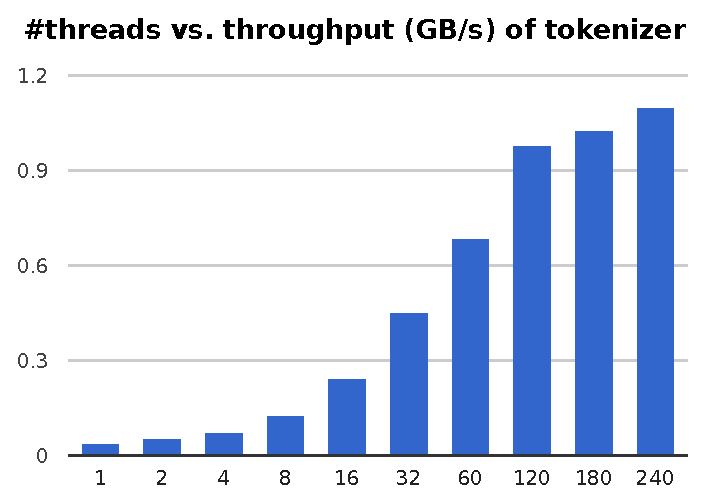
\includegraphics[scale=.66]{img/tokenizer_throughput.eps}
  \caption{Throughput of the tokenizer in GB/s measured with different numbers of threads.
  \label{tokenizer_throughput}}
\end{figure}
The experiments reveal clearly, that the throughput of the tokenizer increases with the number of threads and in Fig.~\ref{tokenizer_throughput} nearly linear scaling can be seen. While the benefits of more threads are significant up to 120 threads, i.e. two threads per core, less performance can be gained from 120 up to 240 threads.

\begin{figure}\centering
  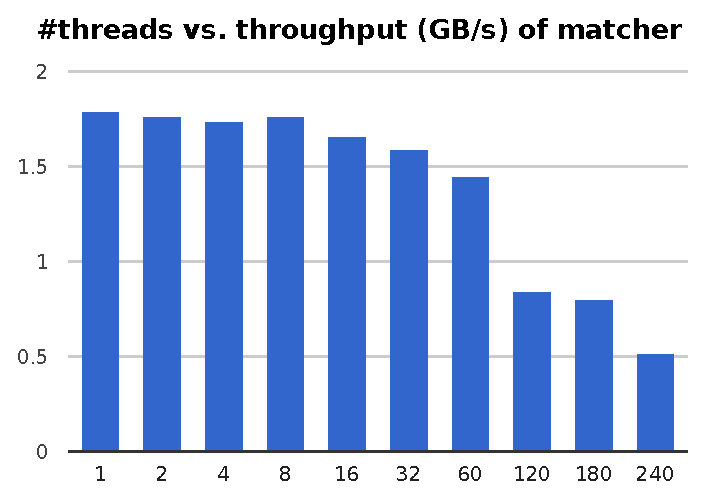
\includegraphics[scale=.66]{img/matcher_throughput.eps}
  \caption{Throughput in GB/s of the matcher with fixed input file size (2GB). Plotted against the number of threads.\label{matcher_throughput}}
\end{figure}
In Fig.~\ref{matcher_throughput} the throughput of the matcher against the numbers of queries, i.e. threads, is plotted. Up to 60 queries there is no significant drop of the performance, while after 120 queries the throughput plummets. Up to 60 threads weak scaling is observable. When the number of threads exceeds the number of cores the performance suffers.

Similarly in Fig.~\ref{matcher_performance} the increase of the processing time after 60 threads can be seen. While the different is not too drastic for files of 2 GB and 4 GB, a spike for 8 GB can be seen. We assume this is due to the memory access pattern of the Xeon Phi, which becomes apparent, when more threads operate at the same time on larger data. Pursuing experiments that confirm this assumption would exceed the format of this report.

\begin{figure}\centering
  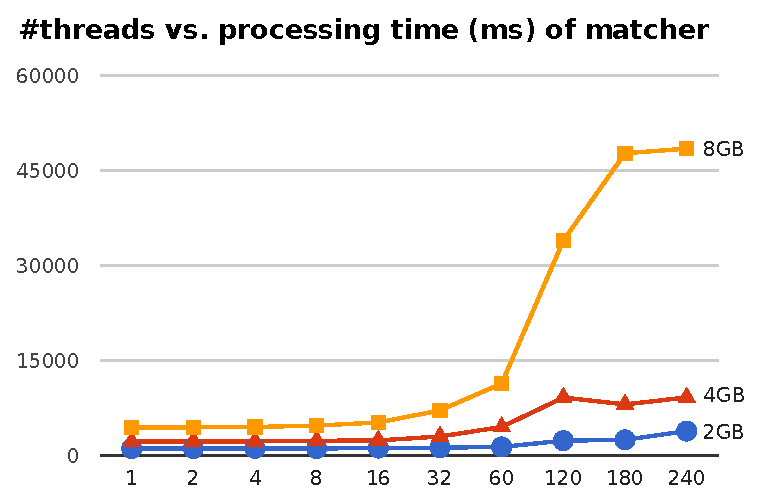
\includegraphics[scale=.66]{img/matcher_processing_time.eps}
  \caption{Processing time of the matcher for 2 GB, 4 GB and 8 GB XML files. Plotted against the number of queries, i.e. threads.\label{matcher_performance}}
\end{figure}
\section{Conclusions}

Here you need to summarize what you did and why this is
important. {\em Do not take the abstract} and put it in the past
tense. Remember, now the reader has (hopefully) read the report, so it
is a very different situation from the abstract. Try to highlight
important results and say the things you really want to get across
such as high-level statements (e.g., we believe that .... is the right
approach to .... Even though we only considered x, the
.... technique should be applicable ....) You can also formulate next
steps if you want. Be brief. After the conclusions there are only the references.


\input{06_appendix.tex}



% References should be produced using the bibtex program from suitable
% BiBTeX files (here: bibl_conf). The IEEEbib.bst bibliography
% style file from IEEE produces unsorted bibliography list.
% -------------------------------------------------------------------------

\bibliography{bibl_conf}
\bibliographystyle{IEEEbib}

\end{document}

